% This is samplepaper.tex, a sample chapter demonstrating the
% LLNCS macro package for Springer Computer Science proceedings;
% Version 2.20 of 2017/10/04
%
\documentclass[runningheads]{llncs}
\usepackage{soul}
\usepackage{tikz}
\usetikzlibrary{calc}
\usepackage{graphicx}


\begin{document}
%
\title{An Event-based Architecture for Cross-Breed Multi-population Bio-inspired Optimization Algorithms}
%
%\titlerunning{Abbreviated paper title}
% If the paper title is too long for the running head, you can set
% an abbreviated paper title here
%
\author{XXXXXXXXXX\inst{1}\orcidID{0000-1111-2222-3333} \and
XXXXXXXXXX\inst{1}\orcidID{1111-2222-3333-4444} \and
XXXXXXXXXX\inst{2}\orcidID{2222--3333-4444-5555}}
%
\authorrunning{XXXXXXXXXX et al.}
% First names are abbreviated in the running head.
% If there are more than two authors, 'et al.' is used.
%
% \institute{National Technological Institute of Mexico
\institute{Hidden institute
\email{XXXXXXXXXX@XXXX.com}\\
%\url{http://www.springer.com/gp/computer-science/lncs}\\
\email{\{abc,lncs\}}}
%
\maketitle              % typeset the header of the contribution
%
\begin{abstract}
  % It seems like the abstract is incompleate, it is a good idea to 
  % write it at the end - Mario
  % You can't present software implementations, but a methodology that
  % you have tested - JJ
  In this work, we present a software implementation that follows an
  event-driven architecture, designed to asynchronously distribute the
  processing of population-based algorithms. The search algorithm uses a
  multi-population approach, creating multiple populations with different
  parameters of execution, allowing the implementation of multiple algorithms, in
  this case Genetic Algorithms (GAs) and Particle Swarm Optimization (PSO).
  Using a message queue, each population is handled by asynchronous
  serverless functions, taking advantage of functional programming
  % "taking advantage of" is not really it. Really, it needs to be
  % that way.
    % \cite{Kunasaikaran2016}
    % No citations in abstract.
    .This cloud-based JavaScript implementation includes a web-based
    application for
    % Why is it cloud ready? - JJ
    the configuration and interaction with algorithms. We executed
    several
    % That's an implementation detail - JJ
    experiments to validate the system, using benchmark functions and
    several configurations. Results show ...

    % Results here 

   % Having
   % the knowledge that both of them are population-based algorithms it can be
   % defined that a migration between 2 or more populations are possible, and
   % this type of hybrid could be helpful to increase the possibility to find the
   % optimal result (the best of the best), there is where fits the concept of
   % Multi-population. 


\keywords{Multi-population  
  \and Asynchronous 
  \and Sub-population 
  \and Serverless 
  \and Distributed.
  \and cross-breed multi-population}
\end{abstract}
%
%
%
\section{Introduction}

In the past few decades, nature-inspired optimization algorithms have been
applied to solve complex real-world problems \cite{yang2014nature}. Algorithms
inspired in natural processes include evolutionary algorithms (EAs)
\cite{back1996evolutionary} and swarm intelligence (SI) \cite{kennedy2006swarm},
among others. These population-based algorithms share the common characteristic
of using an initial set of random candidate solutions that are later used to
generate a new set of candidates, using a nature-inspired heuristic. Popular EAs
are Genetic Algorithms (GAs), Genetic Programming (GP), grey wolf optimization
(GWO) and Differential Evolution (DE), while examples of (SI) are particle swarm
optimization (PSO) and ant colony algorithms (ACO).


As in nature, population-based algorithms
are intrinsically parallel and asynchronous. Because of that, researchers have
been proposing some form of parallelization since the earlier works
\cite{muhlenbein1988evolution} with the objective of increasing the speed of
these algorithms. 
%% Island Model 
One of the first concepts proposed for parallelization was the island model,
which lead to an increased performance \cite{gorges1990explicit,grosso1985computer} 
by dividing a large population into communicated subpopulations.
%% Multi-population 
Since then, the concept has been applied to other population-based algorithms
and has been adapted by researchers to pursue other objectives besides the
execution speed. Currently, researchers use the term multi-population based
methods to describe those techniques using subpopulations as part of their
strategy.


Multi-population based methods divide the original population into
smaller subpopulations or islands, with every subpopulation carrying out the
algorithm independently, with synchronous or asynchronous communication with the
rest of the islands. This relative isolation helps in maintaining an overall
diversity since each subpopulation will search in a particular area, at least
between communications. The recombination mentioned above (mixing) or migration
between subpopulations is needed to avoid a premature convergence of candidate
solutions since smaller populations are known to perform better for a given
problem than bigger populations. However, it gives them the added advantage of
parallel operation. Additionally, and in some cases, multi-population algorithms
scale better than expected due to the interaction between the algorithm and the
paralellism of the operation \cite{ALBA20027}.
% Connect with the idea of heterogeneous populations
However, in most cases, algorithms applied to each subpopulation are
homogeneous, or at any rate, the same variant of the algorithm. As long as this
parallel operation is not synchronous, other population-based algorithms, or, as
a matter of fact, any algorithm, could be easily integrated. That is why several
works based on multi-population are heterogeneous, integrating various
optimization algorithms, and often performing better than single-population or
homogeneous optimization algorithms \cite{wu2016differential,nseef2016adaptive}.
% Explan the proposed method of mixing many algorithms through population streams  


Heterogenous algorithms add another degree of freedom to the problem of finding
the correct parameter settings for an algorithm; because some parameters affect
the accuracy of the solution and the convergence speed of the algorithms as they
tip the balance between exploration and exploitation of the search space. On the
other hand, current studies show that by having a high number of subpopulations
interacting in parallel, the effect of the individual parameters of each
subpopulation is compensated by those selected in other subpopulations. In this
work, we will use random settings within a specific range as results have shown
this is a valid solution to this problem. 
% Two things here 
% * Add references to former work 
% * Explain why some parameters, like the population size, are not
% generated randomly too - JJ 
Some parameters, specialy the population size, are
kept fixed in order to control more easily the execution of the algorithm. For
instance, by having the size of subpopulations fixed, it is easier to control
the number of evaluations and the communication costs, when the algorithm is in
operation.
% 2. State clearly from the beginning, and in a positive way (that is,
% don't use the reasoning: this sucks, so we need something better)
% what is your intention: use a parallel architecture for combined,
% parameter-free-algorithms.
Combining multiple algorithms, with different parameters, interacting with each
other at the same time, can benefit from the strengths of each. For instance, a
genetic algorithm could find a promising global solution that is not optimal
while another algorithm, more suitable for a local search, finds the global
optimum. This approach has been followed extensively in recent years, with
success. Moreover, there is a need for frameworks, architecture, and
implementation models that can allow researchers the development of new
parallel, asynchronous, heterogeneous, and parameter-free algorithms in a scalable way.  

%To deal with these problems, parallel and cross-breed multi-population
%algorithms architecture has been proposed.

% 1. Add more references. Most claims must have a reference to support it.
% 2. State clearly from the beginning, and in a positive way (that is,
% don't use the reasoning: this sucks, so we need something better)
% what is your intention: use a parallel architecture for combined,
% parameter-free-algorithms.
% 3. 

% a paragraph that binds that previous paragraph to our work in this paper. 
%Why is this related to what we presented above? - JJ

In this work, we present a new version of the event-driven architecture proposed
in [Anonymous]; this is a so-called {\em serverless} architecture that
asynchronously processes isolated and heterogeneous subpopulations. Each
subpopulation is treated as an event, that is pushed asynchronously into a
message queue. Events trigger stateless functions that receive the subpopulation
and proceed to run an algorithm, using the paramaters and population included in
the message. After the specified number of iterations, each stateless function
returns the evolved subpopulation by again pushing a message to another queue,
used for receiving the resulting subpopulations. Subpopulations are received
from the queue by a controller that is responsible for mixing the individuals
from different subpopulations and producing new subpopulations. These new
subpopulations are pushed again by the controller into the message queue,
creating a loop. The cycle stops when the controller receives a subpopulation
containing a candidate solution that satisfies a particular condition, or a
maximum number of messages were received. 

In this new version, we propose several improvements to the original. First, we
propose alternative methods of migration between populations to compensate for
differences in the execution time of the functions. The architecture includes
external storage for the subpopulations it receives, instead of an in-process
buffer, that was limited to a small number of sub-populations. Also, the
migration or mixing process includes the capability of doing operations at the
individual-level. 
We can see the proposal as a way of evolving and mixing a
stream of populations that can very different as if their individuals belong to
different species; the term we use to describe the solution is a cross-breed
multi-population method.

% This new
% implementation uses JavaScript for the full stack, and it is designed to be
% executed locally or in a cloud environment. The implementation includes a
% web-based application to execute and monitor experiments
% interactively. % implementation detail, best left for the conclusions
               % - JJ
%We also
%propose alternative methods of migration between populations to compensate for
%differences in the execution time of the functions. % This is probably
                                % one of the main points of the
                                % paper. Should be enphasized more
                                % - JJ

%%%%% BEGIN (needs work)

To evaluate the capability of a cross-breed multi-population solution,
we conducted several experiments using different benchmark functions, comparing the
results of single versus cross-breed multi-population algorithms. For the experiments, we choose to
compare the PSO and GA algorithms, as they are well understood, and there are
several implementations in the literature. We implemented both algorithms as
stateless functions, and more algorithms can be added in the same way.

%%%%% END (needs work): - Mario

%%
%% A description of the paper goes here
%% what are we proposing? You can start with the description in the abstract.  
%% what are the findings? 
%% what is presented in each section? 
%% Check other papers to get the idea - Mario

The rest of the paper is organized as follows: the next section is devoted
to analyzing the state of the art of multi-population, multi-paradigm,
stateless evolutionary algorithms. The architecture proposed is
presented in Section \ref{sec:architecture} and put to work in Section\ref{sec:exp}.
Finally, we present our conclusions and future lines of work.

\section{State of the Art}

% The title of these subsections will be removed, they are just place-holders
% References are pending
%\subsection{Multi-population}

Multi-population based methods have been used extensively in recent years, with
some journal papers dedicated exclusively to surveying the current state of the
art \cite{ma2019multi} and challenges \cite{li2015multi}. A recent survey on
ensemble strategies for population-based optimization algorithms
\cite{wu2019ensemble} reports current advances on parametrization and
implementation techniques, presenting results in competitive and collaborative
multi-populations as well as parametrization techniques.

Multi-population techniques are heavily applied in dynamic optimization, from
island-based parallel EAs \cite{lissovoi2017runtime}, harmony search
\cite{turky2014multi} and ACO \cite{nseef2016adaptive}. Combinatorial problems
\cite{pourvaziri2014hybrid}, using a combination of local and global operators
\cite{bai2018integrated}.

Then there are also surveys dedicated to reporting current advances in the
parallelization of particular population-based heuristics, from parallel PSO
\cite{Lalwani2019}, using GPUs in particular \cite{tan2015survey} , ACO
\cite{pedemonte2011survey} and distributed EAs \cite{gong2015distributed}.  


\subsection{Parallel, Distributed}
The most common form of paralellization is to exploit the capabilities of multi-core CPUs and
GPUs.   




Distributed and cloud-based architectures are used extensively in the software
industry because of their high performance and lower overall cost. Many systems
are being created and migrating step by step to microservices and new serverless
architectures, which proposes the use of Function as a Service (FaaS) 
\cite{Hellerstein2018,Everywhere,Baird2016}. 
Researchers are starting to exploit this type of architectures in heuristic optimization
development, and here we take advantage of them to increase the performance of
some population-based algorithms.

\subsection{Cloud, Serverless}
% These sections can be optional, 
% they can be part of the Intro, SoA, of a Concepts section - Mario

% Multi-population
% Parallel, Distributed 
% Cloud
% Serverless

Recently, cloud providers such as Amazon Web Services (AWS), IBM Cloud, and
Google Cloud, offers a new alternative to programming through interfaces called
Serverless Computing [References], this platform consists of an effortless a
mechanism where developers upload the code into the platform and execute it as
many times as it is required, scaling and allowing to do this in parallel. This
way, the developers do not worry about servers, connections, and other
configurations. In serverless, users pay only for what it is used. There is also
the option to install some of these platforms locally; for instance, AWS (Amazon
Web Services) \cite{Baird2016} or Apache Open Whisk \cite{Guerv2018}. 


% \begin{figure}[htp]
%   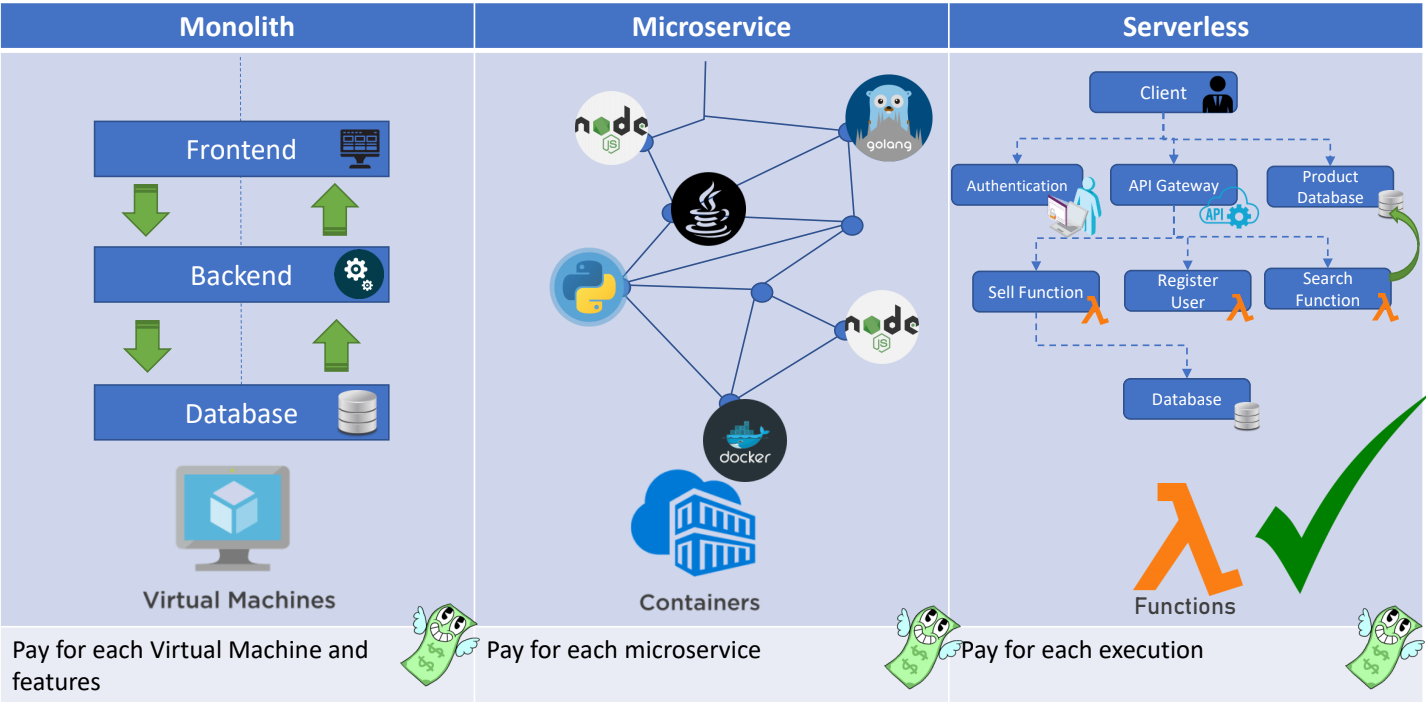
\includegraphics[width=\textwidth]{img/architectures.png}
%   \caption{Software architecture generations.} \label{fig1}
%   \end{figure}
\begin{table}[htp]
  \caption{Software architecture generations.}
  \label{table:architectures}
  \centering
  \begin{tabular}{|c|c|c|c|}
  \hline
  Monolitic & Microservices & Serverless \\
  \hline
  Pay for each virtual  & Pay for each  & Pay for each \\
  machine and features & microservice & execution \\
  \hline
  Composed by a model  & Composed by virtual containers & Composed by functions \\
  Client-Server-Database & that execute small parts of a system & inside containers \\
  \hline
  Inside Virtual Machines & Inside Containers & Cluster of functions\\
  \hline
  Require Operator System & Not Operator System required & Not Operator System required\\
  \hline
  \end{tabular}
  \end{table}





\subsubsection{Serverless Operation} 
In math, a function is a relation between a set of inputs and an allowed set of
outputs, with the idea that each input goes to a single output. However, in
computer science, a function is defined as a unit of code that has a role in a
greater code structure, works on various inputs that usually are variables and
throws a concrete output that is the result of the process those variables. One
of the main features that belong to functions is that they are stateless, they
are focused on inputs and result with a simple process that does not require a
state, at the moment the inputs get into the function are already generating an
output. In serverless, events such as messages or HTTP requests can trigger
these functions. Also, each function scales independently and is stateless with
a short duration \cite{Baird2016,Cook2017}.
% I am not a fan of that definition of a function in CS - Mario
% Explain a bit more the "Stateless" part - Mario 

\subsection{Asynchronous}

Asynchronous algorithms consist of performing a certain action such as the
movement of the particles in PSO or the crosses and mutations of the GA without
the need for the execution of one to affect the other, in a few words a
Individual execution of each without waiting times. This is very useful. when
several threads are used in parallel execution because if the expected response
of action, for example, a GA of 100 generations and a GA of 10 is it is
preferable not to stop the search and give priority to 10 generations
\cite{Santander-jim2018,Sherry2012,Goebel2016,Guerv2018}. Asynchronous functions
are created in programming that has promising results response that is immediate
and does not stop the main execution by secundary actions
\cite{Moroney2017,Ambler2015}.

An asynchronous architecture has what is known as execution queues in the that
can be appreciated that give an added value that gives advantage over other
architectures by reducing waiting times and neglecting the concept that order is
important, of course, this type of architectures is not applicable to all cases
but speaking in distributed systems where multiple population-based algorithms
are executed with parallel execution, they result in a better degree of
efficiency, in addition to reducing the number of control parameters since they
require having a decoupled architecture \cite{Ma2019,Santander-jim2018}.

\subsection{Functional Programming}

It is a very important programming paradigm that is based on lambda expression,
created from math knowledge. The programming languages could be classified by
programming styles, there are usually known as programming paradigms
\cite{Kunasaikaran2016}.

In the functional programming style the data does not exist independently or by
themselves, but these happen in the form of arguments and are transformed as a
flow in an exit through the functions. Each function is described as atomic
because each one only has a simple operation that generates an expected result
\cite{Kunasaikaran2016}.


\section{Proposed architecture}
\label{sec:architecture}

The proposal is an architecture that allows processing of a single population
that is divided into sub-populations, distributing them to processes in different
ways, and then communicating with each other with the purpose of increasing the
possibility to find the highest fitness of a function. This architecture can accept
the use of an indeterminate number of algorithms, allowing an easy cross-breed multi-population 
and continuous adaptability for different problems. % A reference to a
                                % figure should go around here - JJ

% Before nodes, you need to explain the overall layout of the
% architecture - JJ
This architecture consist in 3 nodes, % Nodes or types of nodes?
they are explained on the next points:

\begin{itemize}
  \item {\bf Manager}: This node creates a population conformed by sub-populations is created and the architecture
  initialize parameters to run the algorithm. Every time a sub-population is
  created triggers an event that sends the subpopulations to be stored in a 
  JSON file into the MongoDB data store (preventing to saturate the
  memory) % what do you mean here? - JJ
  and to a message queue
  that is directed to its subsequent processing in the “Receiver” section that
  is our cluster of functions (Faas), because each sub-population requires the
  execution of a different algorithm, there is a different channel in the web
  sockets for each type of algorithm that triggers its respective serverless
  function. Once a subpopulation is processed, it is returned and a selection is
  made for the sub-population migration. The migration selection is made by
  taking the population attribute of the subpopulation that was returned and the
  subpopulation that it has been selected among the best 2, it should be noted
  that the decision to identify the best from the 2 is made randomly. Once the
  selection is made, a Splitting Point Uniform crossing will be made. The 2 new
  subpopulations replace their self and are resent it back to their respective
  serverless function and this process is repeated until completing the number
  of assigned migrations for the multi-population
  \cite{Ma2019,Santander-jim2018}. Of course this whole process is performed
  asynchronously avoiding the wait for all responses from serverless functions
  to perform a crossover or an update of the multi-population status
  \cite{Lovbjerg2001,Jimeno2019}. In the following figure, you can see from the
  illustrative way how the multi-population is composed.
% \begin{figure}[htp]
%   \centering
%   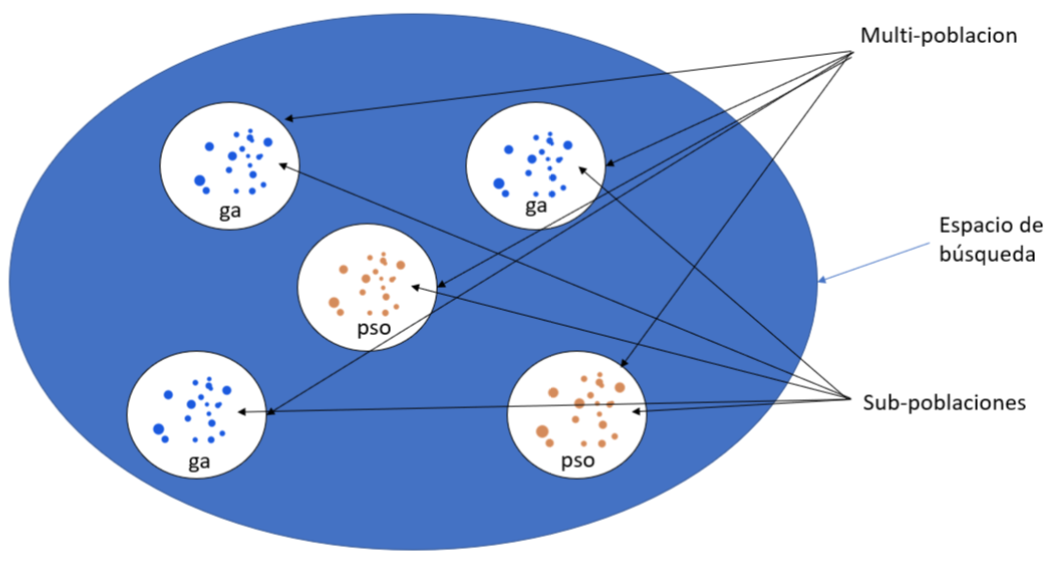
\includegraphics[width=0.7\textwidth]{img/multipopulation.png}
%   \caption{Multipopulation representation.} \label{fig1} %This is defined twice. 
%   \end{figure}
  The mechanism to send the sub-population to the serverless functions is
 creating a queue with a dimension of 2 positions that asynchronously allow
 communicating.
\item {\bf Message Provider}: Its purpose is the creation of a sub-population messages
  queue which is the communication channel % A queue is not a channel,
                                % it's _in_ a channel - JJ
  between the sub-population Manager and
the Receiver (FaaS), each message is a trigger for the execution of a GA or PSO
function. Thanks to the message queue, it is possible to perform the serverless
functions asynchronously, avoiding waiting states in the algorithm
while responses arrive, 
independently of their duration and the simultaneous evaluation of different
sub-populations independent of its algorithm or characteristics.
\item Receiver: Here are the Serverless
  functions of the % which section? Are you talking about the receiver
                   % itself? - JJ
algorithms to be executed, reducing the best possible using the functional
programming paradigm so that they can be converted into FaaS without problems,
in addition to achieving a completely clean and fast
execution\cite{Roberts2016}. Each message received on this node is executed in
the form of a multi-threaded process in parallel, this allows having more than
one population-based search algorithm running at the same time and making a copy
of itself each algorithm functions as required.
\end{itemize}

To develop this architecture the applied technologies are based in JavaScript
using Node JS as it can be seen in the General Architecture Flowchart
shown in Figure \ref{fig2}.

% I don't think this figure is appropriate for a paper.
\begin{figure}[htp]
  \centering
  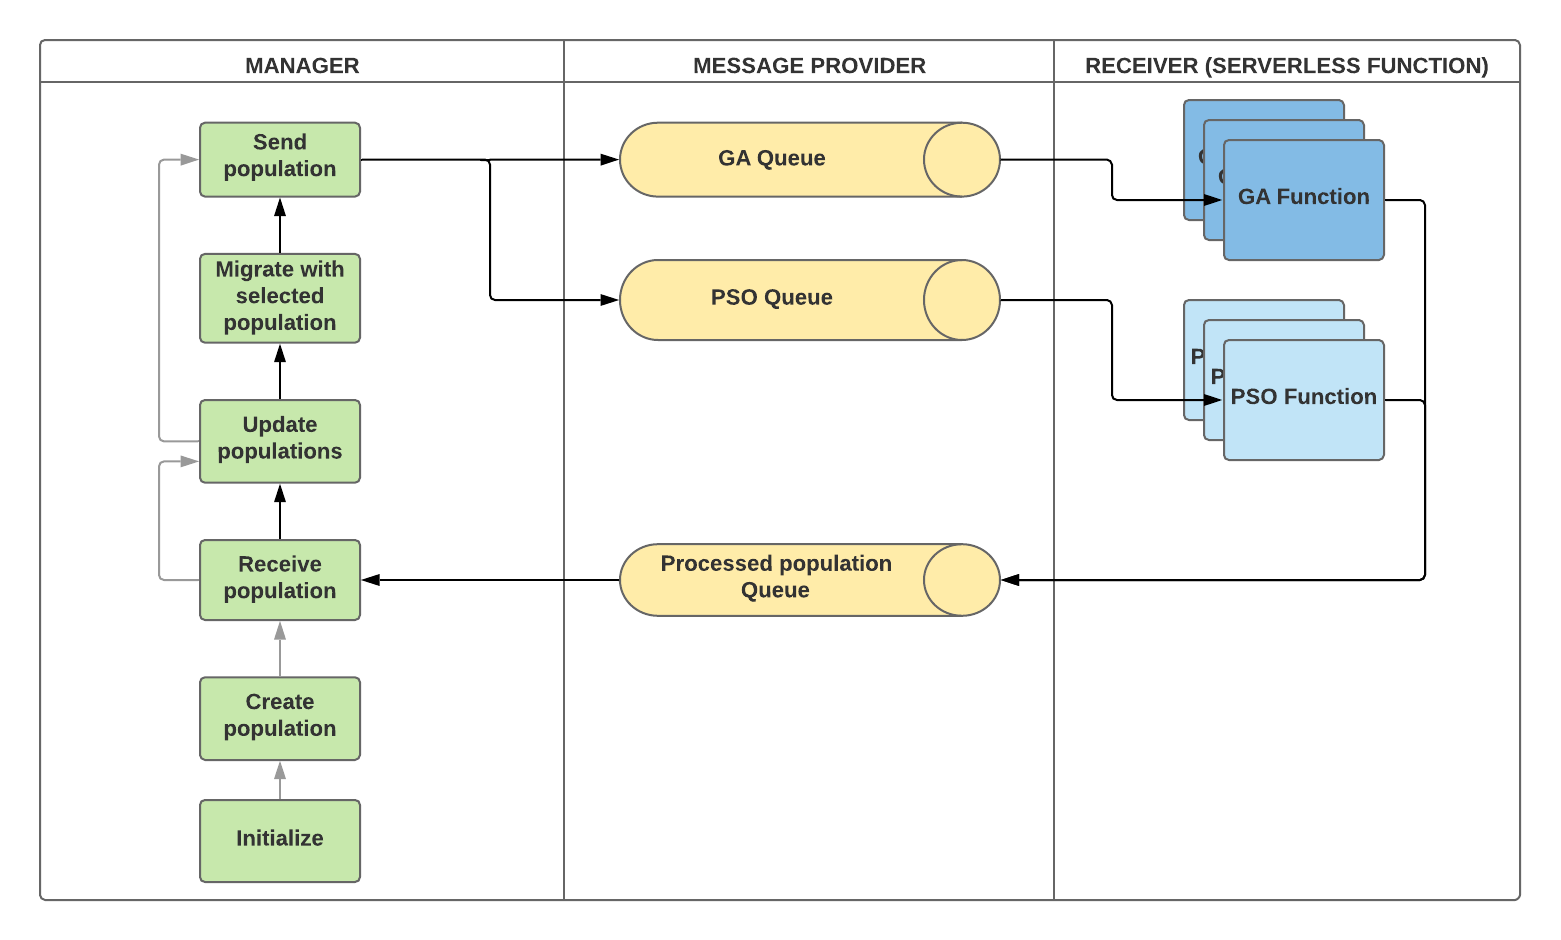
\includegraphics[width=0.9\textwidth]{img/Architecture diagram.png}
  \caption{General Architecture Flowchart.} \label{fig2}
  \end{figure}
  % Could be OK for the presentation, divided in 3 slides - JJ
  
\subsection{Sub-population definition}

Individuals are created composed of 2 types of information, the one that is
active or useful for crossing and the one that is not. % this is not a
                                % proper definition. - JJ
The population contains
the series of possible solutions, while the rest % what is the rest? -
% JJ
% Please rewrite this - JJ
contains the information on how
the processing for the search of the optimal solutions will be executed, linked
directly with their respective algorithms.
Y
\begin{figure}[htp]
  \centering
  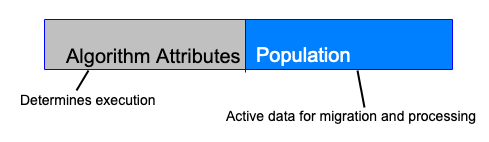
\includegraphics[width=0.6\textwidth]{img/subpopulationDefinition.png}
  \caption{Sub-population composition.} \label{fig3}
  \end{figure}

\subsection{Splitting Point Uniform Migration}

This architecture communicates sub-populations using migrations,
taking
% It's not an architecture, unless you mean the overall architecture - JJ
information from 2 sub-populations and mixing them using a process similar to a
crossover in Genetic Algorithms, creating 2 completely new sub-populations every
time a processed sub-population arrives into the Manager node and replacing
themselves in the multi-population.

The migration created to % to? For? - JJ
this architecture is a method called Splitting Point
Uniform that consists of a uniform mask that is created to apply the migration
between individuals, vectors or both of them, from two sub-populations. The
selected data are combined using the midpoint between the active values
points by the binary mask generated randomly. % Not clear. Maybe a
                                % picture? - JJ
This process iterates the 2
sub-populations to randomly swap values and replaces some of them with middle
points \cite{Kramer2017,Kaya2011}.


\begin{figure}[htp]
  \centering
  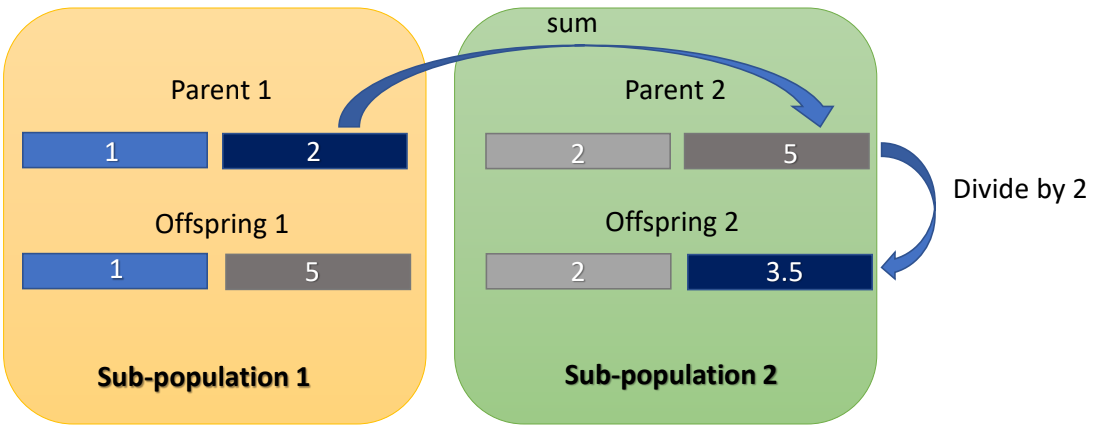
\includegraphics[width=0.9\textwidth]{img/splittinPointUniform.png}
  \caption{Splitting Point Uniform process.} \label{fig4}
  \end{figure}

  \subsection{Migration Selection} The 2 sub-populations selected to realize
  migration is one arrived sub-population from a serverless function and another
  one using selection by tournament keeping up the information of the best
  sub-population of the multi-population but without discarding possible
  sub-populations that in a near future could be the clue to find optimal
  values.

\begin{figure}[htp]
  \centering
  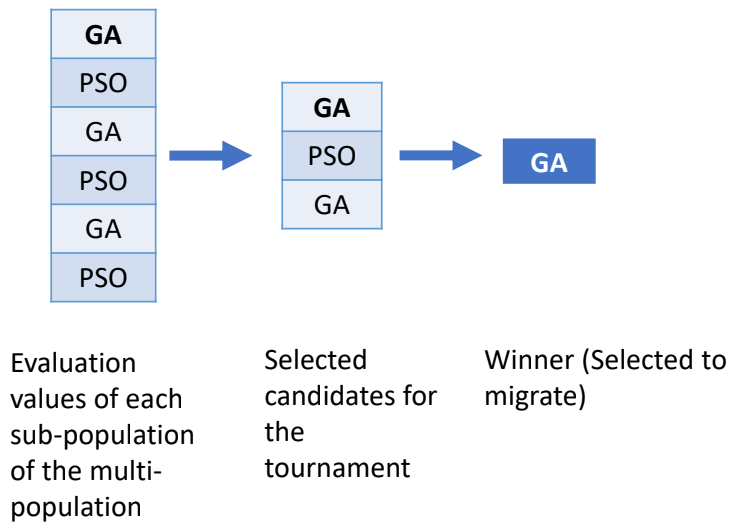
\includegraphics[width=0.5\textwidth]{img/selection.png}
  \caption{Selection by tournament.} \label{fig5}
  \end{figure}


  \section{Experiments and Results}
  \label{sec:exp}

  In this section we will first present the experiments that have been
  made, including the configuration of parameters that has been used,
  to then proceed to present and discuss the results in Subsection
  \ref{subs:results}. 
    
  \subsection{Experiments}

With the configuration shown in the section above, we performed a
series of runs to check that results obtained were, at least, similar
to similar estups, and we were satisfied with them; we need to prove,
however, they obtain a good performance on benchmark functions, and
what is their relative performance in a controlled environment.

% ----------------- This intro eliminated ---------------------------------
% Now that interaction between sub-populations with different algorithms is
% working and cross-breed multi-population has been a success, using until now the added
% algorithms (GA and PSO) algorithms \cite{Kramer2017,Guerrero2017,Lalwani2019},
% all thanks to the developed architecture, let's proceed to the
% experiments.
% --------------------------------------------------------------------------
%
\begin{figure}[htp]
  \centering
    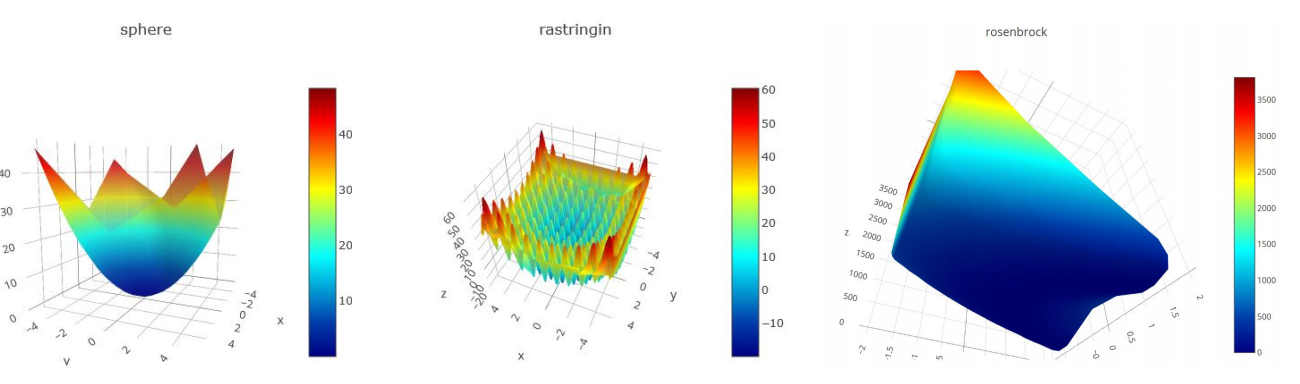
\includegraphics[width=0.7\textwidth]{img/benchmark.png}
    \caption{Benchmark functions for experimentation.} \label{fig:functions}
    \end{figure}
%
First, we will select the functions we are going to apply this
framework to. We will be working on continuous optimization, since
they are hard optimization problems and have also been chosen for
benchmarks such as BBOB \cite{hansen2010bbob}; out of these functions,
we have chosen Rastrigin, Sphere and Rosenbrock, which are represented
in Figure \ref{fig:functions}. They have a different
degree of difficulty, can be scaled to different dimensions (as all
the rest of the benchmark functions), and they can at least give us an
idea of how single-breed (GA or PSO) algorithms perform compared to
our cross-breed (GA+PSO) version.
%

   \begin{table}[h!tp]
    \caption{Parameters used by the algorithms for all dimensions. The Random mutation for GA includes the Tournament2, Tournament3, Random, RandomLinearRank, Sequential, Fittest variants. Fitness function is minimized in both cases.}
    \label{table:ga-pso-parameters}
    \centering
    \begin{tabular}{|l|c|c|}
    \hline
    Parameter & \multicolumn{2}{c|}{Values for dimensions} \\
      \hline
      & 2 & 10, 20, 40 \\
    \hline
    GA Generations & 50 &  70\\
    \hline
     GA Population size & 100 & 200\\
    \hline
    GA Mutation &  \multicolumn{2}{c|}{Random}\\
    \hline
    GA Crossover selection & \multicolumn{2}{c|}{Tournament3} \\
    \hline
    GA Crossover percentage & \multicolumn{2}{c|}{Random[10\%, 80\%]} \\
    \hline
    GA Mutation percentage & \multicolumn{2}{c|}{Random[10\%,50\%]} \\
    \hline
    GA Crossover function & \multicolumn{2}{c|}{1 point crossover} \\
    \hline
    GA Mutation Function & \multicolumn{2}{c|}{Gaussian} \\
      \hline 
      \hline
    PSO Iterations & 50 & 70\\
    \hline
    PSO Vector size & 100 & 200\\
    \hline
    PSO Social factor & \multicolumn{2}{c|}{Random[0.5,4.0]} \\
    \hline
    PSO Individual factor & \multicolumn{2}{c|}{Random[0.5,4.0]} \\
    \hline
    PSO Inercia factor & \multicolumn{2}{c|}{Random[0.5,4.0]} \\
    \hline
    \end{tabular}
\end{table}

The parameters used for these algorithms are shown in table
\ref{table:ga-pso-parameters}. In every algorithm run, we will use  a
stop criteria of an error below 0.5E-8. The cross-breed algorithm
itself used 10 sub-populations for each
experiment and a maximum of 4 migrations per sub-population..
Since this was intended mainly
as a first approach to the performance of the cross-breed algorith, we
did not perform any kind of optimization in the parameter space. Note
that we use random parametrization for every population, except for
the number of iterations before migration takes place and the vector
size (in the case of PSO) % Please clarify what's this vector size, I
                          % have no idea - JJ
or population size (in the case of the GA). We kept these number
fixed, and also did not vary it except for the smallest case
(dimensions = 2). This was made mainly for the sake of a fair
comparison between two algorithms, but in principle, and as a line of
research we could approach in the future, this could also be either
random or adaptive depending on the number of dimensions.

The maximum number of evaluations follows this equation:
\begin{equation}
    \label{eq:hesitancy-interpretation}
   Evaluations = 10^{5} Dimensions
   \end{equation}
This means that evaluations will scale from 200K for the 2 dimensions,
un to 4 millions for 4 dimensions.  This kind of parametrization is
also usual in benchmarks, but of course we could use different
parameters depending on the function and scaling in a different, and
non-linear, way. 

Every experiment was carried out 15 times, using % way which kind of
                                % computer and operating system was
                                % used, as well as the code, if it's
                                % been released. Please add answer to
                                % #17 here.

\subsection{Results}
\label{subs:results}
%
\begin{table}[h!tp]
  \caption{2,10,20,40 dimensional experiment result averages}
  \label{table:resultados-2}
  \centering
% latex table generated in R 3.4.4 by xtable 1.8-2 package
% Thu Nov 14 13:02:26 2019
\begin{tabular}{rllrrr}
  \hline
Dimensions & Algorithm & Function & Average & SD & Best \\ 
  \hline
  2 & GA-PSO & Rastrigin & 0.00E+00 & 0.00E+00 & 0.00E+00 \\ 
  2 & GA-PSO & Rosenbrock & 6.91E-09 & 1.57E-08 & 9.58E-14 \\ 
  2 & GA-PSO & Sphere & 4.33E-14 & 1.37E-13 & 0.00E+00 \\ 
  2 & GA & Rastrigin & 1.65E-08 & 1.94E-08 & 0.00E+00 \\ 
  2 & GA & Rosenbrock & 1.24E-08 & 2.27E-08 & 1.62E-13 \\ 
  2 & GA & Sphere & 4.37E-10 & 1.17E-09 & 4.53E-18 \\ 
  2 & PSO & Rastrigin & 1.89E-12 & 7.31E-12 & 0.00E+00 \\ 
  2 & PSO & Rosenbrock & 2.48E-06 & 9.59E-06 & 1.12E-12 \\ 
  2 & PSO & Sphere & 7.80E-12 & 2.06E-11 & 0.00E+00 \\ 
  3 & GA-PSO & Rastrigin & 7.72E-09 & 2.40E-08 & 0.00E+00 \\ 
  3 & GA-PSO & Sphere & 6.28E-10 & 2.39E-09 & 0.00E+00 \\ 
  3 & GA & Rastrigin & 1.21E-08 & 1.98E-08 & 9.98E-13 \\ 
  3 & GA & Sphere & 4.20E-11 & 1.41E-10 & 1.74E-15 \\ 
  3 & PSO & Rastrigin & 0.00E+00 & 0.00E+00 & 0.00E+00 \\ 
  3 & PSO & Sphere & 3.30E-11 & 1.18E-10 & 0.00E+00 \\ 
  5 & GA-PSO & Rastrigin & 5.57E-08 & 1.71E-07 & 0.00E+00 \\ 
  5 & GA-PSO & Sphere & 8.68E-09 & 1.74E-08 & 0.00E+00 \\ 
  5 & GA & Rastrigin & 1.27E-08 & 1.48E-08 & 4.68E-12 \\ 
  5 & GA & Sphere & 5.89E-09 & 8.62E-09 & 4.41E-11 \\ 
  5 & PSO & Rastrigin & 6.54E-01 & 1.71E+00 & 0.00E+00 \\ 
  5 & PSO & Sphere & 1.48E-03 & 5.74E-03 & 0.00E+00 \\ 
  10 & GA-PSO & Rastrigin & 5.09E-09 & 1.15E-08 & 8.01E-12 \\ 
  10 & GA-PSO & Rosenbrock & 2.40E-04 & 4.63E-04 & 3.62E-07 \\ 
  10 & GA-PSO & Sphere & 1.30E-09 & 2.67E-09 & 3.34E-11 \\ 
  10 & GA & Rastrigin & 2.38E-06 & 5.86E-06 & 3.22E-09 \\ 
  10 & GA & Rosenbrock & 1.67E-04 & 2.88E-04 & 9.58E-07 \\ 
  10 & GA & Sphere & 2.54E-08 & 2.13E-08 & 1.84E-09 \\ 
  10 & PSO & Rastrigin & 2.72E+00 & 3.87E+00 & 7.86E-11 \\ 
  10 & PSO & Rosenbrock & 4.43E+00 & 1.07E+01 & 4.17E-07 \\ 
  10 & PSO & Sphere & 3.08E-02 & 1.19E-01 & 4.50E-11 \\ 
  20 & GA-PSO & Rastrigin & 7.38E-02 & 2.58E-01 & 9.13E-09 \\ 
  20 & GA-PSO & Rosenbrock & 5.61E-03 & 5.85E-03 & 2.32E-05 \\ 
  20 & GA-PSO & Sphere & 2.13E-08 & 2.95E-08 & 9.11E-11 \\ 
  20 & GA & Rastrigin & 2.21E-01 & 4.30E-01 & 8.09E-04 \\ 
  20 & GA & Rosenbrock & 1.10E-02 & 1.71E-02 & 3.48E-04 \\ 
  20 & GA & Sphere & 9.23E-06 & 7.55E-06 & 1.85E-06 \\ 
  20 & PSO & Rastrigin & 2.55E+01 & 4.04E+01 & 3.99E+00 \\ 
  20 & PSO & Rosenbrock & 1.34E+01 & 3.68E+00 & 9.12E+00 \\ 
  20 & PSO & Sphere & 3.50E-07 & 9.46E-07 & 7.04E-11 \\ 
  40 & GA-PSO & Rastrigin & 2.13E+00 & 1.83E+00 & 2.46E-04 \\ 
  40 & GA-PSO & Rosenbrock & 5.25E-01 & 4.71E-01 & 1.85E-02 \\ 
  40 & GA-PSO & Sphere & 1.41E-04 & 3.63E-04 & 2.00E-10 \\ 
  40 & GA & Rastrigin & 3.56E+00 & 1.47E+00 & 1.95E+00 \\ 
  40 & GA & Rosenbrock & 1.07E+02 & 1.66E+02 & 3.29E+01 \\ 
  40 & GA & Sphere & 5.30E-03 & 1.85E-03 & 2.69E-03 \\ 
  40 & PSO & Rastrigin & 1.30E+02 & 1.12E+02 & 2.91E+01 \\ 
  40 & PSO & Rosenbrock & 3.68E-01 & 3.28E-01 & 3.27E-02 \\ 
  40 & PSO & Sphere & 2.07E-03 & 8.01E-03 & 8.68E-11 \\ 
 
  \end{tabular}
  \end{table}
  

    
      % \begin{figure}[htp]
      %   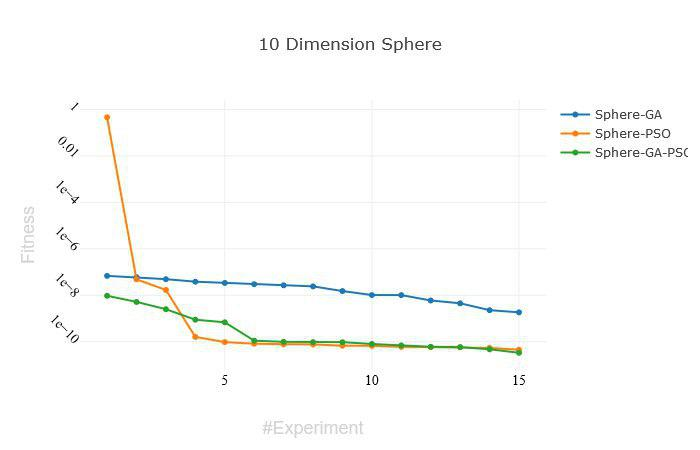
\includegraphics[width=\textwidth]{img/10-sphere.jpg}
      %   \caption{10 dimensions experiments Sphere.} \label{fig10}
      %   \end{figure}

      %   \begin{figure}[htp]
      %     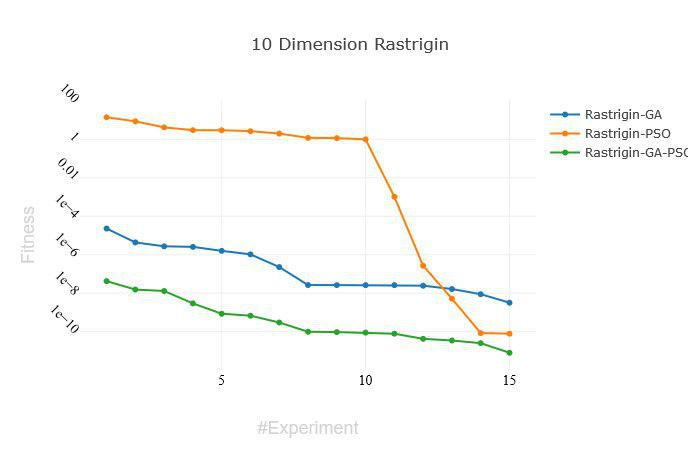
\includegraphics[width=\textwidth]{img/10-rastrigin.jpg}
      %     \caption{10 dimensions experiments Rastrigin.} \label{fig11}
      %     \end{figure}

      %     \begin{figure}[htp]
      %       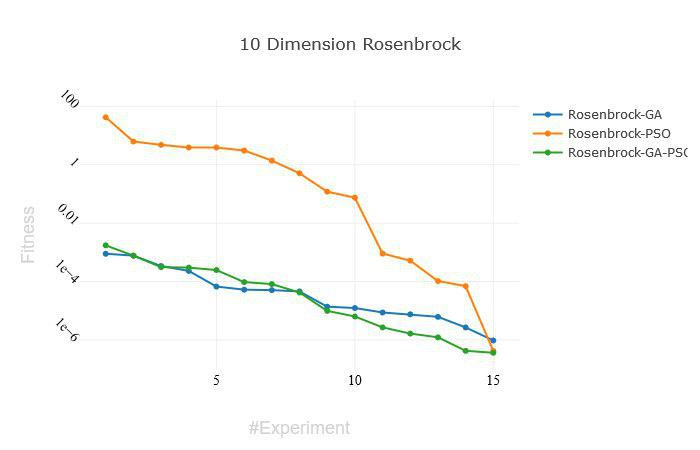
\includegraphics[width=\textwidth]{img/10-rosenbrock.jpg}
      %       \caption{10 dimensions experiments Rosenbrock.} \label{fig12}
      %       \end{figure}

    
          
            % \begin{figure}[htp]
            %   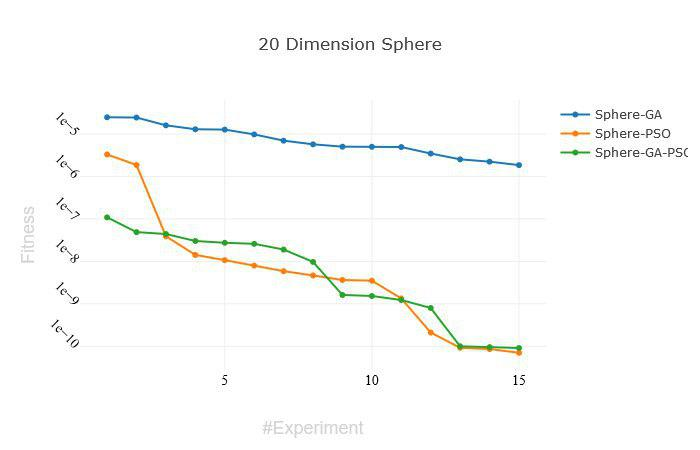
\includegraphics[width=\textwidth]{img/20-sphere.jpg}
            %   \caption{20 dimensions experiments Sphere.} \label{fig13}
            %   \end{figure}
      
            %   \begin{figure}[htp]
            %     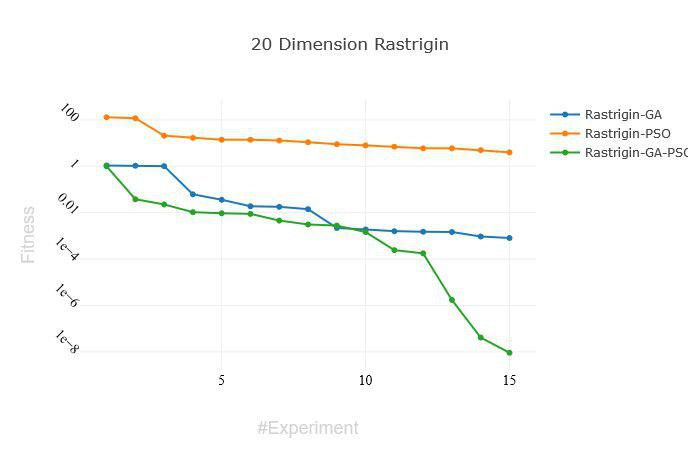
\includegraphics[width=\textwidth]{img/20-rastrigin.jpg}
            %     \caption{20 dimensions experiments Rastrigin.} \label{fig14}
            %     \end{figure}
      
            %     \begin{figure}[htp]
            %       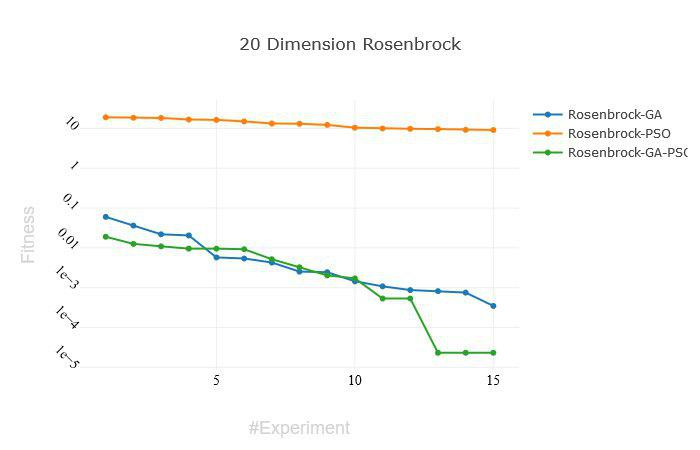
\includegraphics[width=\textwidth]{img/20-rosenbrock.jpg}
            %       \caption{20 dimensions experiments Rosenbrock.} \label{fig15}
            %       \end{figure}

       
    
      % \begin{figure}[htp]
      %   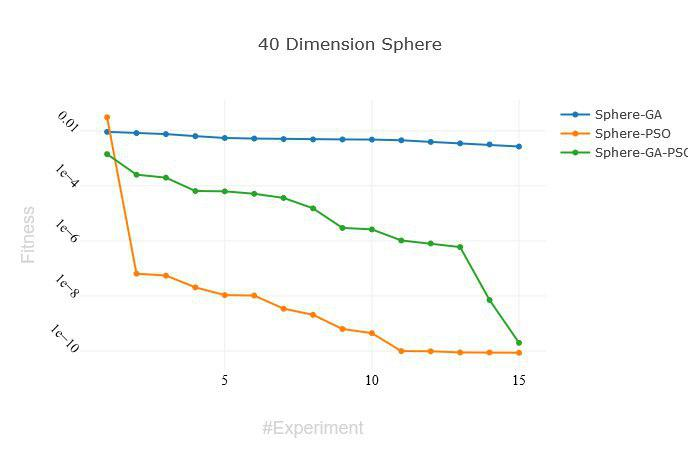
\includegraphics[width=\textwidth]{img/40-sphere.jpg}
      %   \caption{40 dimensions experiments Sphere.} \label{fig1}
      %   \end{figure}

      %   \begin{figure}[htp]
      %     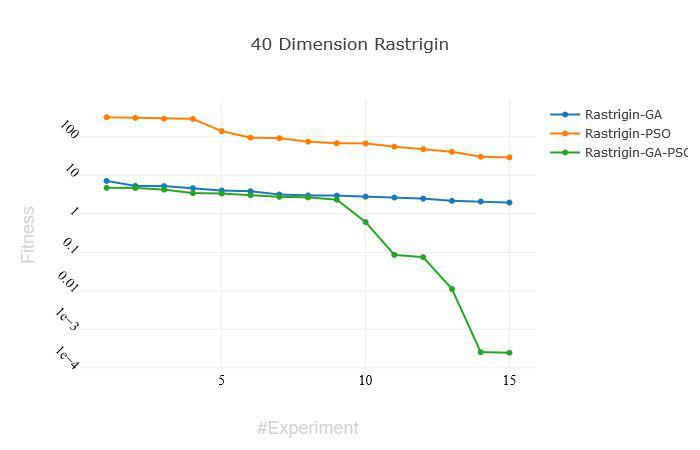
\includegraphics[width=\textwidth]{img/40-rastrigin.jpg}
      %     \caption{40 dimensions experiments Rastrigin.} \label{fig1}
      %     \end{figure}

      %     \begin{figure}[htp]
      %       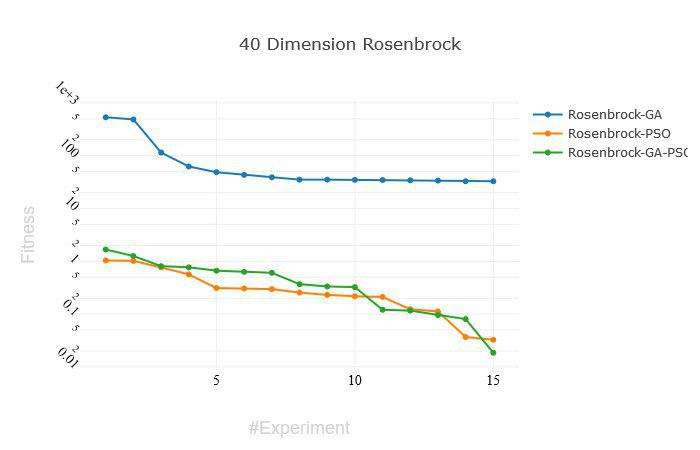
\includegraphics[width=\textwidth]{img/40-rosenbrock.jpg}
      %       \caption{40 dimensions experiments Rosenbrock.} \label{fig1}
      %       \end{figure}


    
            \begin{figure}[h!tb]
              \centering
                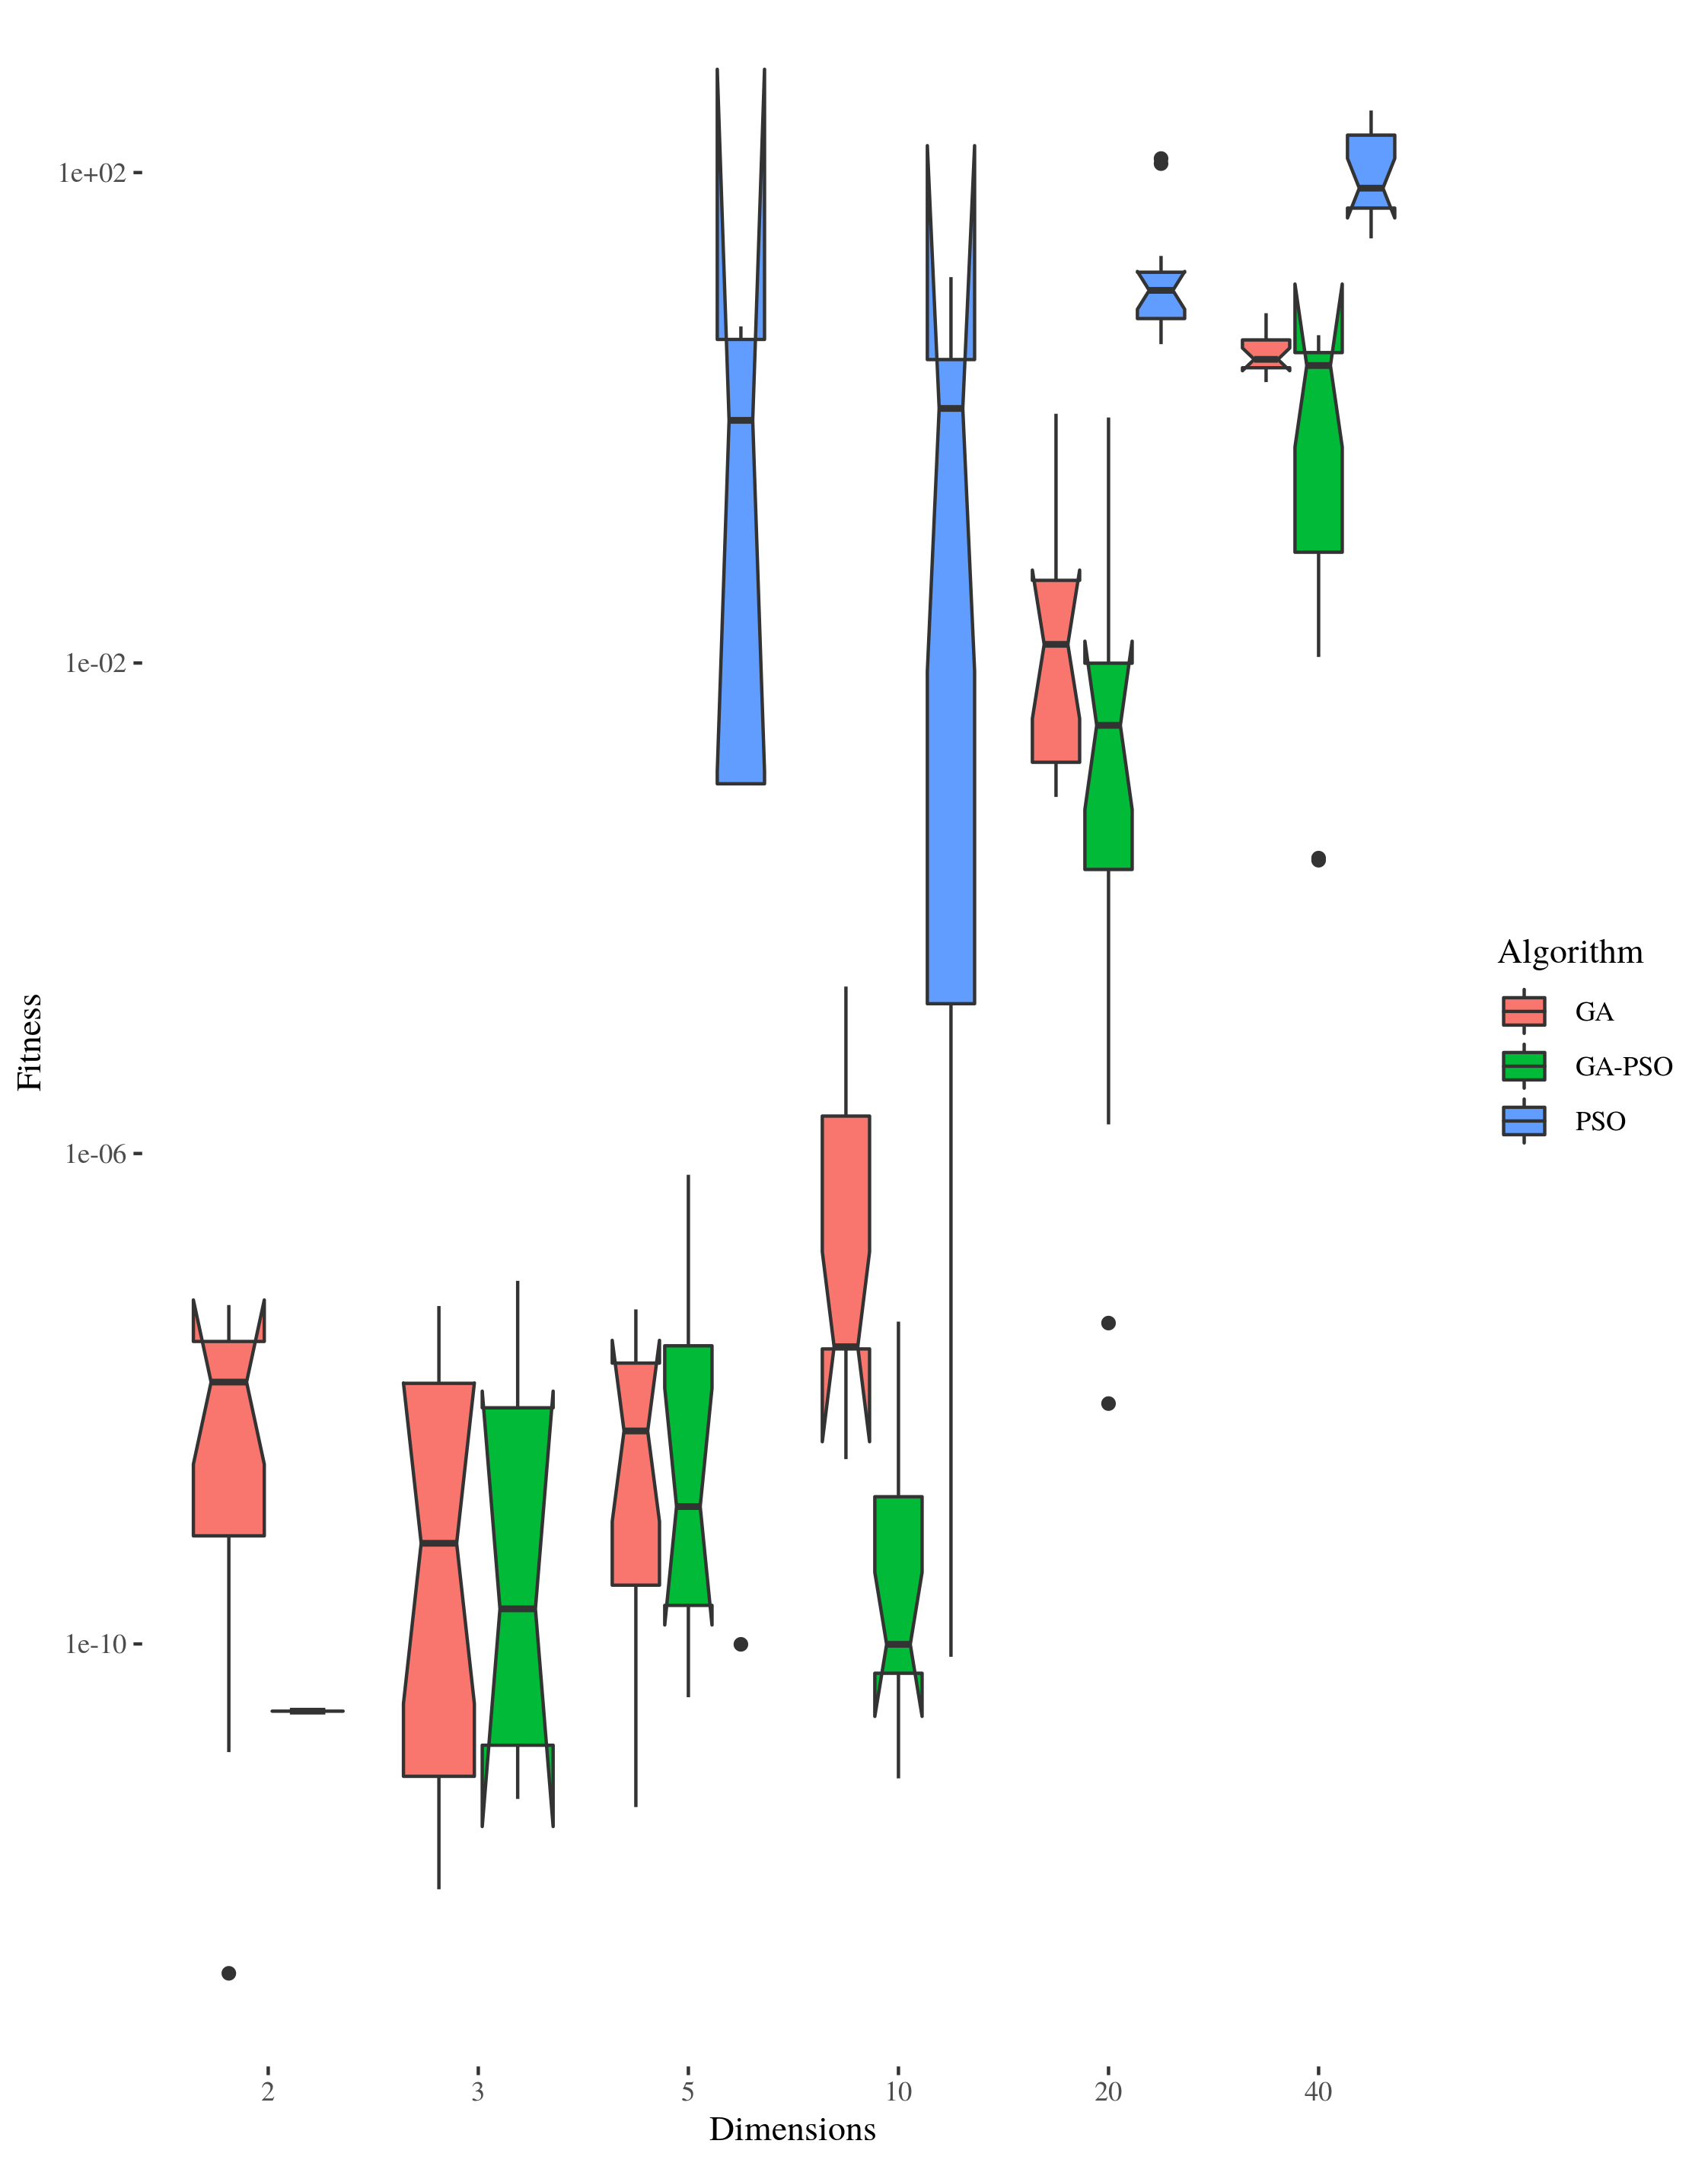
\includegraphics[height=0.5\textheight]{img/rastrigin-boxplot.png}
              \caption{Boxplot of results for Rastrigin function. Please note the $y$ axis is logarithmic..\label{fig:boxplot:rastrigin}}
            \end{figure}
%
                 \begin{figure}[h!tb]
              \centering
                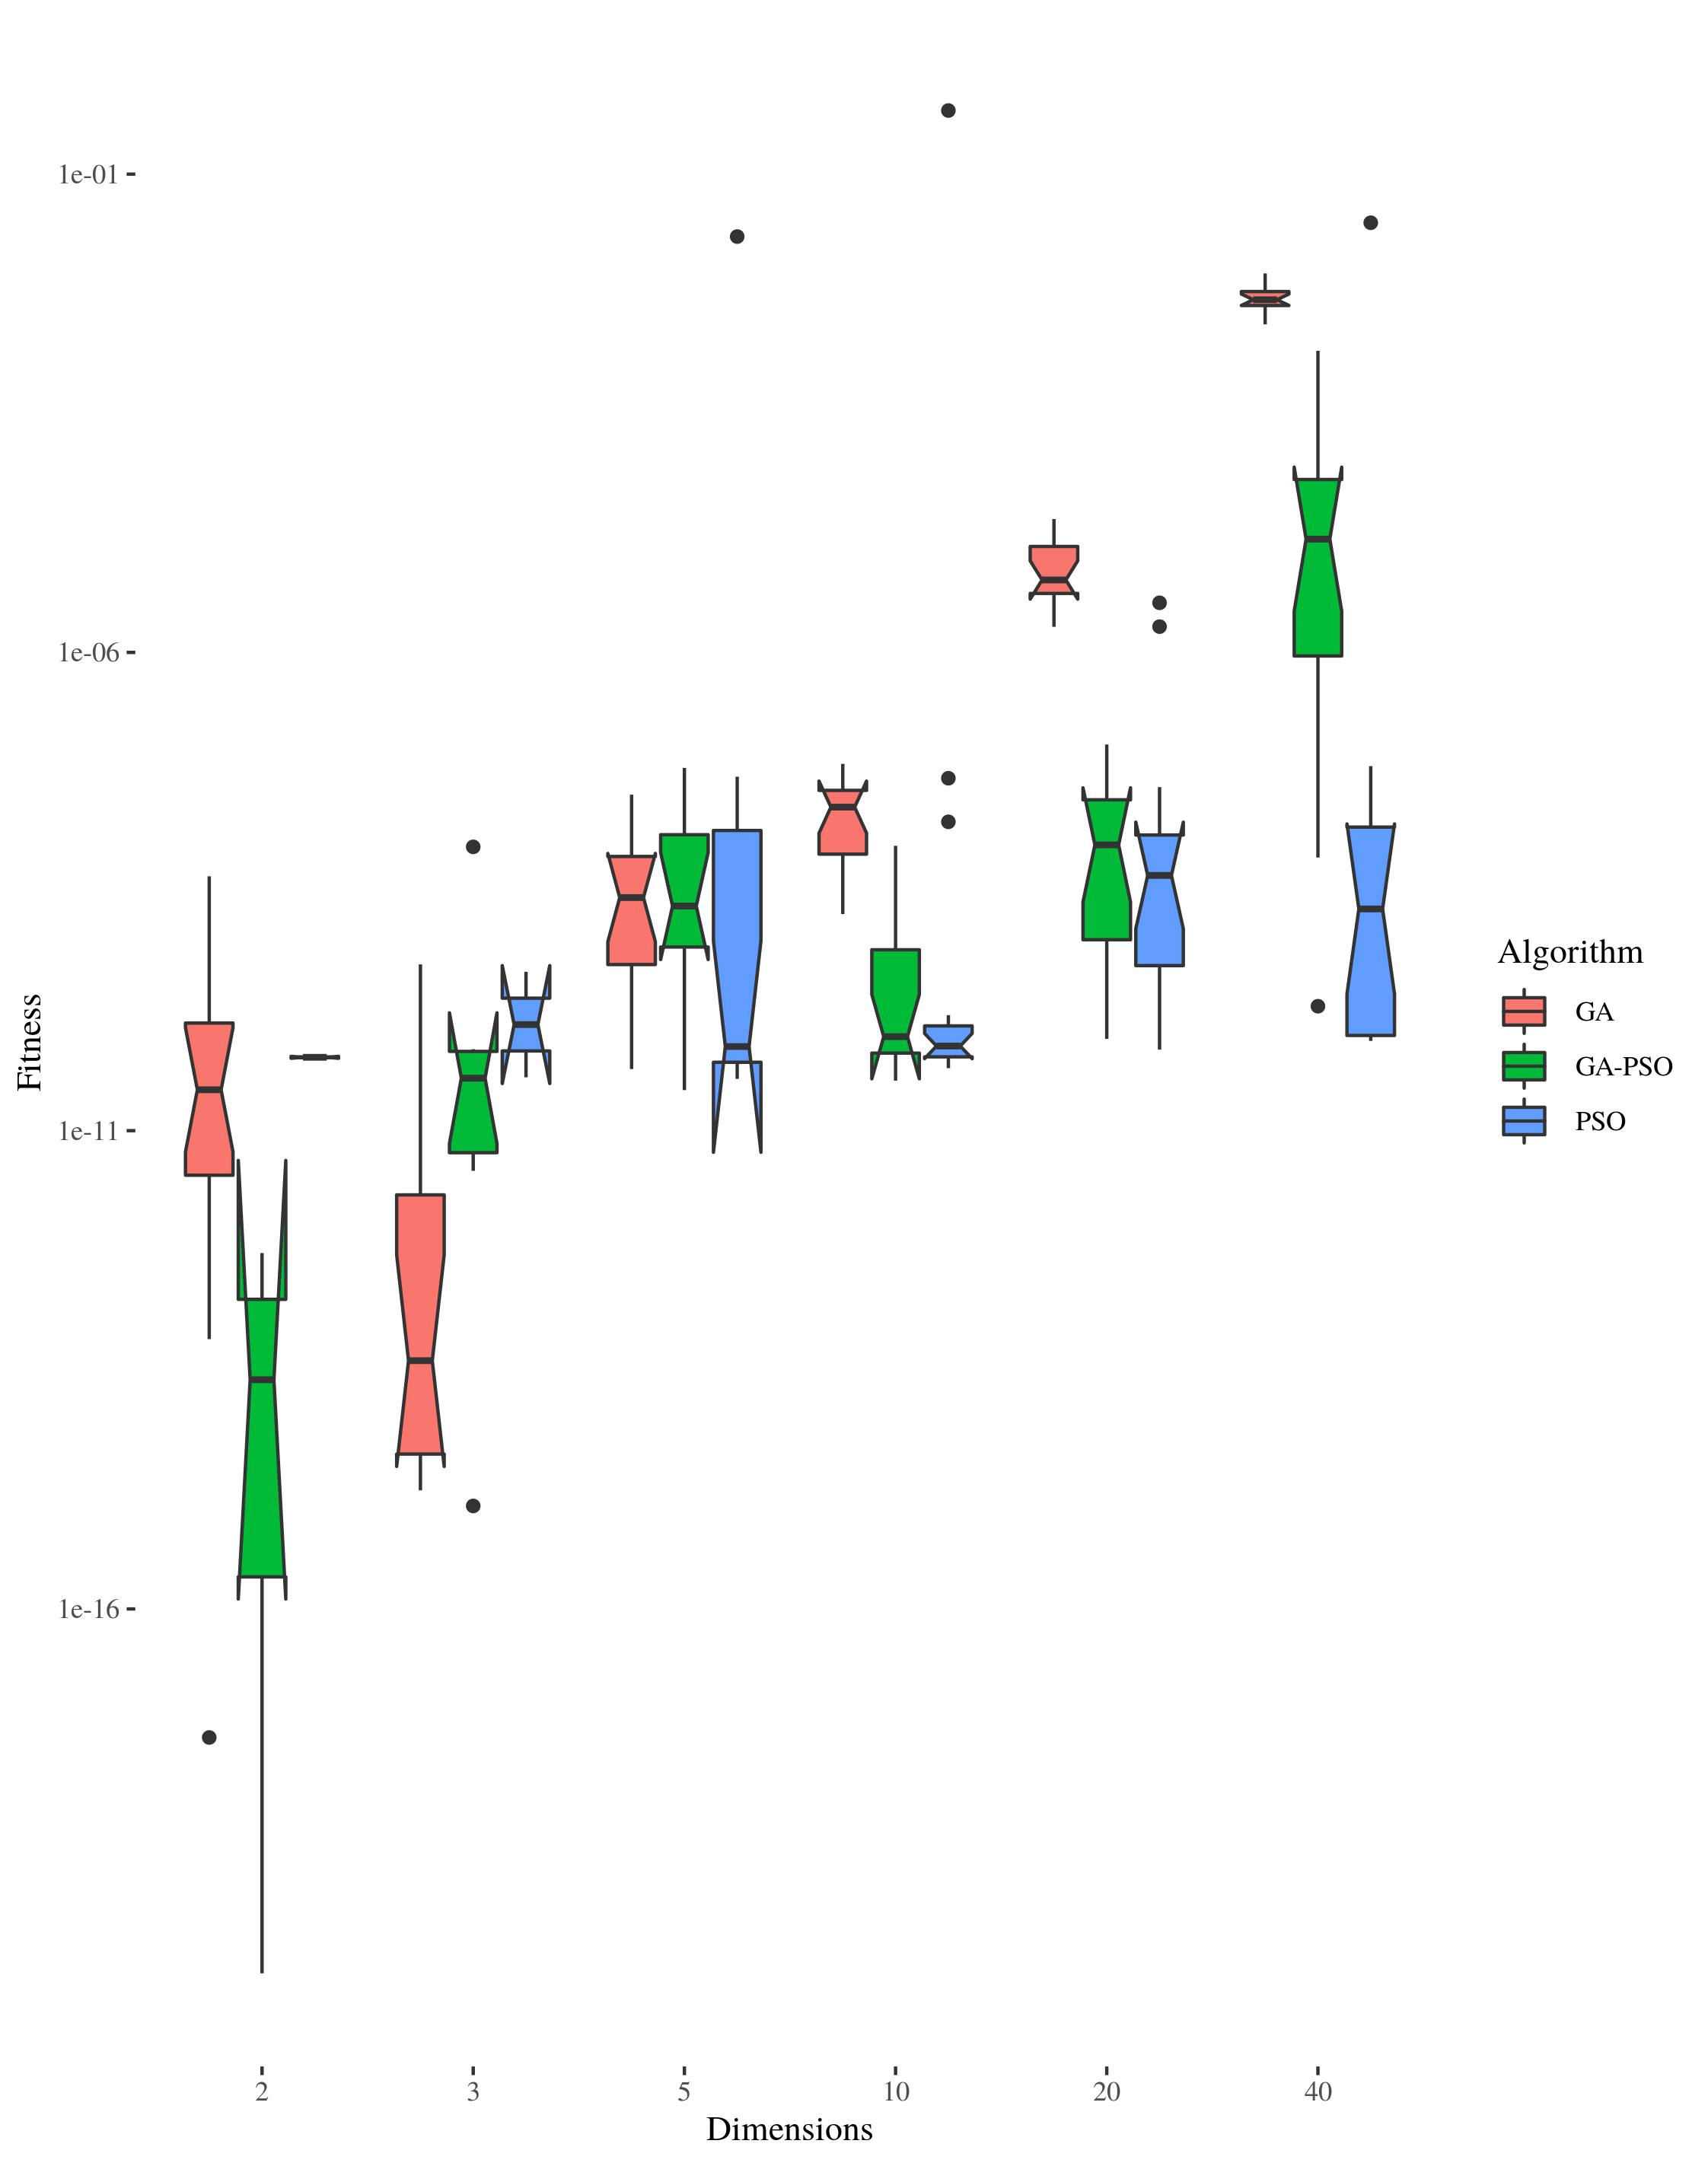
\includegraphics[height=0.5\textheight]{img/sphere-boxplot.png}
              \caption{Boxplot of results for the Sphere function, with a logarithmic $y$ axis.\label{fig:boxplot:sphere}}
            \end{figure}
%
                 \begin{figure}[h!tb]
              \centering
                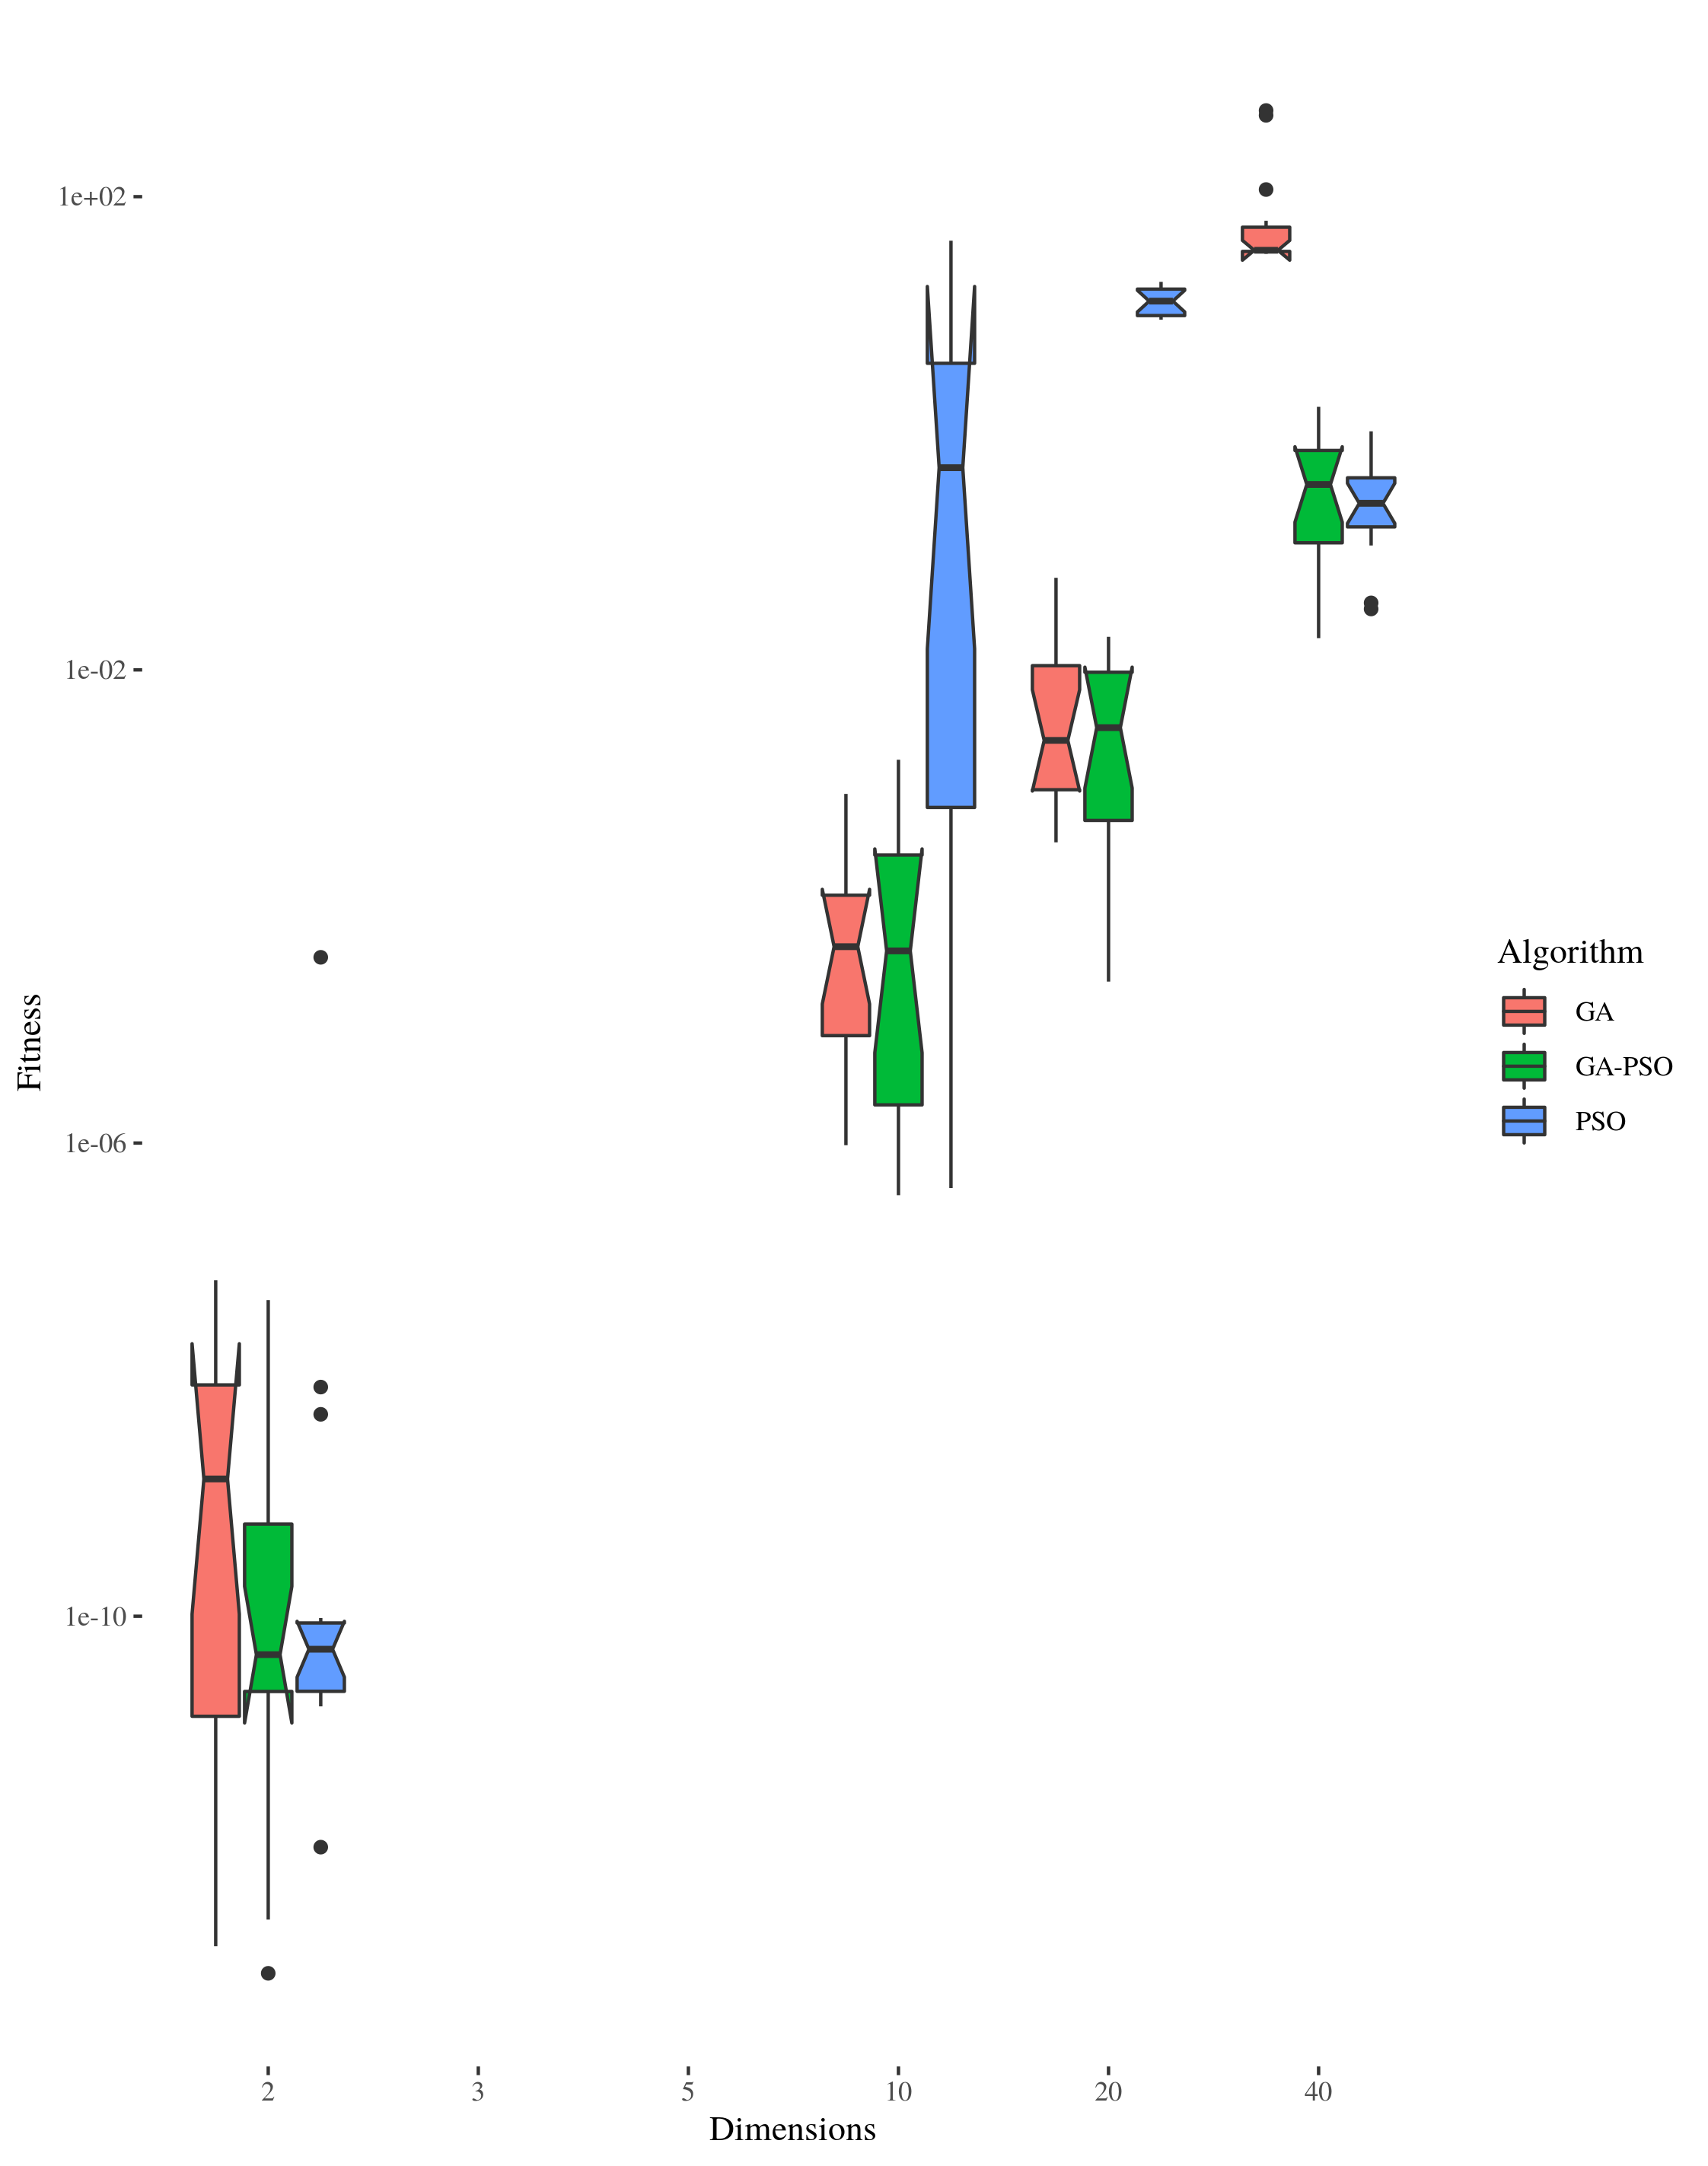
\includegraphics[height=0.5\textheight]{img/rosenbrock-boxplot.png}
              \caption{Boxplot of results for the Rosenbrock function; $y$ axis is logarithmic.\label{fig:boxplot:rosenbrock}}
            \end{figure}
            
\section{Conclusions and future work}

This architecture is completely scalable and useful for implementation of
multiple algorithms, until now is only GA and PSO but according to the results
with this kind of architecture there is no limit and it works better than
cross-breed multi-population with only one algorithm, also every experiment executes in
short times because serverless functions searching in an asynchronous way
getting a fast convergence.

%\section{Future work}

% Reference with interesting challenges: li2015multi 
% Dynamic optimization needs: a non-fixed number of populations, 
% how to increase (measure) diversity in dynamic optimization problems.
% restrict or not restrict populations in certain areas.

To get a continuous improvement it is believed that it is required a sort of
mutation applied to the sub-populations. This mutation would be a swapping type,
taking the algorithm parameters from the best and the worst sub-populations,
increasing the possibilities to get an optimal result, preventing get stuck into
a local optimum. Of course, it is expected to use this architecture using more
algorithms than GA and PSO.

% Maybe add randomizing all elements of the population, including
% population and number of generations - JJ

\section*{Acknowledgements}

Acks\\
taking this much\\
space

\bibliography{multipopulation}
      \bibliographystyle{ieeetr}
  
\end{document}
